\documentclass[border=5pt]{standalone}
\usepackage[T1]{fontenc}
\usepackage{lmodern}
\usepackage{pgfplots}
\usepgfplotslibrary{groupplots}
\pgfplotsset{compat=1.18}
\begin{document}\sffamily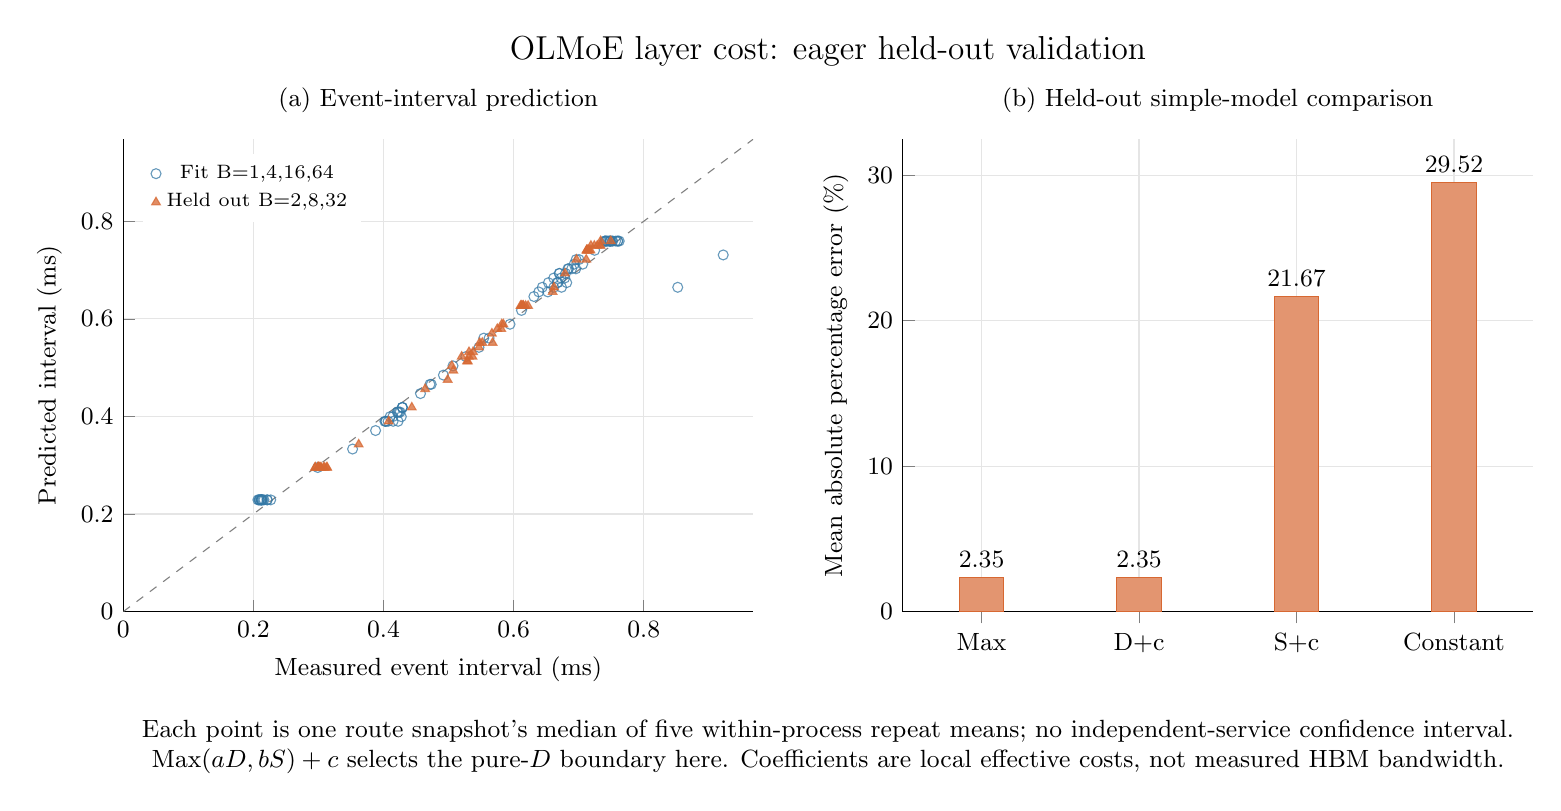
\begin{tikzpicture}
\definecolor{cal}{HTML}{3478A5}\definecolor{test}{HTML}{D76832}\definecolor{profile}{HTML}{3B8A5A}
\begin{groupplot}[group style={group size=2 by 1,horizontal sep=1.9cm},width=8.0cm,height=6.0cm,scale only axis,axis lines*=left,grid=major,grid style={gray!20},tick label style={font=\small},label style={font=\small},title style={font=\small},legend style={font=\scriptsize,draw=none},unbounded coords=jump]
\nextgroupplot[title={(a) Event-interval prediction},xlabel={Measured event interval (ms)},ylabel={Predicted interval (ms)},xmin=0,xmax=0.9682142391800881,ymin=0,ymax=0.9682142391800881,legend pos=north west]\addplot[only marks,color=cal,mark=o,mark size=1.8pt,opacity=0.75] coordinates {(0.22658719942,0.229026319143) (0.208918400854,0.229026319143) (0.216217599809,0.229026319143) (0.298867200315,0.295320645136) (0.220980799198,0.229026319143) (0.211860799789,0.229026319143) (0.352425600588,0.333203117131) (0.214593599737,0.229026319143) (0.213196800649,0.229026319143) (0.387755201757,0.371085589127) (0.212102400512,0.229026319143) (0.209734400362,0.229026319143) (0.428855997324,0.418438679122) (0.21236319989,0.229026319143) (0.211548800021,0.229026319143) (0.456782397628,0.446850533118) (0.208526399732,0.229026319143) (0.206836798787,0.229026319143) (0.473342399299,0.465791769116) (0.221439999342,0.229026319143) (0.212230399251,0.229026319143) (0.492043198645,0.484733005114) (0.406988801062,0.390026825125) (0.422368000448,0.390026825125) (0.425468802452,0.408968061123) (0.471355202794,0.465791769116) (0.41412320137,0.399497443124) (0.428947201371,0.418438679122) (0.506742401421,0.503674241112) (0.410091201961,0.399497443124) (0.428809601068,0.418438679122) (0.55405279994,0.560497949105) (0.403428801894,0.390026825125) (0.42381439954,0.408968061123) (0.594376003742,0.588909803102) (0.403401598334,0.390026825125) (0.427371199429,0.399497443124) (0.526428803802,0.52261547711) (0.401993601024,0.390026825125) (0.421087999642,0.408968061123) (0.546692794561,0.541556713108) (0.414697599411,0.390026825125) (0.422134400904,0.408968061123) (0.562203198671,0.560497949105) (0.65246720314,0.655204129095) (0.666876801848,0.674145365093) (0.667841598392,0.674145365093) (0.693008005619,0.712027837088) (0.643964791298,0.664674747094) (0.653422397375,0.674145365093) (0.669958403707,0.69308660109) (0.638572797179,0.655204129095) (0.661577600241,0.683615983091) (0.696049597859,0.721498455087) (0.631094402075,0.645733511096) (0.67051999867,0.69308660109) (0.700459203124,0.721498455087) (0.612041607499,0.617321657099) (0.689166399837,0.702557219089) (0.922108799219,0.730969073086) (0.852195200324,0.664674747094) (0.69554399848,0.702557219089) (0.724463996291,0.740439691085) (0.661611199379,0.664674747094) (0.706128001213,0.712027837088) (0.740921598673,0.759380927083) (0.762283194065,0.759380927083) (0.673619195819,0.664674747094) (0.748959997296,0.759380927083) (0.759932807088,0.759380927083) (0.681568005681,0.674145365093) (0.740067198873,0.759380927083) (0.760014396906,0.759380927083) (0.678494405746,0.683615983091) (0.752212804556,0.759380927083) (0.747118398547,0.759380927083) (0.672719997168,0.683615983091) (0.742334401608,0.759380927083) (0.756771203876,0.759380927083) (0.679673591256,0.69308660109) (0.745060798526,0.759380927083) (0.748292800784,0.759380927083) (0.684363201261,0.702557219089) (0.743080002069,0.759380927083) (0.748273596168,0.759380927083) (0.683358392119,0.702557219089) (0.740342396498,0.759380927083) (0.751080000401,0.759380927083)};
\addlegendentry{Fit B=1,4,16,64}
\addplot[only marks,color=test,mark=triangle*,mark size=1.8pt,opacity=0.75] coordinates {(0.312614402175,0.295320645136) (0.294828797877,0.295320645136) (0.303404797614,0.295320645136) (0.361838400364,0.34267373513) (0.299817602336,0.295320645136) (0.295201598108,0.295320645136) (0.407924798131,0.390026825125) (0.304014402628,0.295320645136) (0.3079279989,0.295320645136) (0.443449600041,0.418438679122) (0.298977597058,0.295320645136) (0.298998400569,0.295320645136) (0.464006400108,0.456321151117) (0.300743998587,0.295320645136) (0.313380801678,0.295320645136) (0.498584002256,0.475262387115) (0.309545600414,0.295320645136) (0.300188797712,0.295320645136) (0.507216003537,0.494203623113) (0.301311999559,0.295320645136) (0.299884802103,0.295320645136) (0.53764000237,0.532086095109) (0.531257605553,0.52261547711) (0.546708804369,0.541556713108) (0.551824000478,0.551027331107) (0.574902394414,0.579439185103) (0.531377604604,0.532086095109) (0.547708800435,0.551027331107) (0.614486399293,0.626792275098) (0.528395205736,0.513144859111) (0.567692798376,0.551027331107) (0.659926399589,0.655204129095) (0.52950399518,0.513144859111) (0.566545602679,0.569968567104) (0.661955198646,0.664674747094) (0.536774396896,0.52261547711) (0.580956795812,0.579439185103) (0.678908798099,0.69308660109) (0.520083200932,0.52261547711) (0.581702402234,0.588909803102) (0.696520003676,0.721498455087) (0.5049616009,0.503674241112) (0.584193608165,0.588909803102) (0.7180768013,0.740439691085) (0.713055998087,0.740439691085) (0.6125135988,0.626792275098) (0.711583998799,0.721498455087) (0.715764802694,0.740439691085) (0.615019202232,0.626792275098) (0.715815997124,0.740439691085) (0.712049606442,0.740439691085) (0.614302399755,0.626792275098) (0.71313919723,0.740439691085) (0.712292793393,0.740439691085) (0.611724799871,0.626792275098) (0.712748801708,0.740439691085) (0.718748798966,0.749910309084) (0.610571199656,0.626792275098) (0.724057596922,0.749910309084) (0.733592003584,0.749910309084) (0.618393599987,0.626792275098) (0.728457599878,0.749910309084) (0.73373760879,0.759380927083) (0.622190400958,0.626792275098) (0.732566398382,0.749910309084) (0.749311992526,0.759380927083)};
\addlegendentry{Held out B=2,8,32}\addplot[gray,dashed,forget plot,domain=0:0.9682142391800881] {x};
\nextgroupplot[title={(b) Held-out simple-model comparison},ylabel={Mean absolute percentage error (\%)},ybar,bar width=16pt,xtick={1,2,3,4},xticklabels={Max,D+c,S+c,Constant},ymin=0,xmin=0.5,xmax=4.5,nodes near coords,point meta=y,every node near coord/.append style={font=\small,/pgf/number format/fixed,/pgf/number format/precision=2}]\addplot[fill=test!70,draw=test] coordinates {(1,2.34505968362) (2,2.34505968362) (3,21.6729336849) (4,29.5165256885)};
\end{groupplot}
\path (group c1r1.north west) -- node[above=0.8cm,font=\large] {OLMoE layer cost: eager held-out validation} (group c2r1.north east);
\path (group c1r1.south west) -- node[below=1.25cm,align=center,font=\small] {Each point is one route snapshot's median of five within-process repeat means; no independent-service confidence interval.\\Max$(aD,bS)+c$ selects the pure-$D$ boundary here. Coefficients are local effective costs, not measured HBM bandwidth.} (group c2r1.south east);
\end{tikzpicture}\end{document}
